\chapter{Fundamentação Teórica e Trabalhos Relacionados}

Neste capítulo são discutidos os conceitos básicos ao entendimento deste trabalho, abrangendo aprendizagem de máquina, processamento digital de imagens, segmentação de imagens e extração de características.

\section{Aprendizagem de máquina e reconhecimento de padrões}

Conforme \citeonline{alpaydin:2010}, aprendizagem de máquina é uma área da inteligência artificial que estuda métodos computacionais, a fim de obter um determinado conhecimento específico através de experiências. A aplicação prática de aprendizado de máquina inclui o processamento de linguagem natural, diagnósticos médicos, detecção de intrusos, entre outros. Um sistema de aprendizado tem a função de analisar informações e generalizá-las, para a extração de novos conhecimentos.

Segundo \citeonline{russell:2010}, os tipos de aprendizagem podem ser classificados de acordo com o tipo de \textit{feedback} que recebem do ambiente:

\begin{itemize}
    \item \textbf{Aprendizagem não-supervisionada}: o agente aprende padrões na entrada, embora não seja fornecido nenhum \textit{feedback} explícito. A tarefa mais comum de aprendizagem não-supervisionada é o agrupamento, ou seja, a detecção de grupos de exemplos de entrada potencialmente úteis.
    \item \textbf{Aprendizagem por reforço}: também conhecida como aprendizagem semi-supervisionada. O agente aprende a partir de uma série de reforços - recompensas ou punições.
    \item \textbf{Aprendizagem supervisionada}: o agente observa alguns exemplos de pares de entrada e saída, e aprende uma função que faz o mapeamento da entrada para a saída. 
\end{itemize}

Os problemas de aprendizagem podem ainda ser divididos de acordo com o tipo de saída que demandam:

\begin{itemize}
	\item \textbf{Problemas de classificação}: quando a saída esperada para o problema é uma classe ou categoria, ou seja, um valor discreto;
	\item \textbf{Problemas de regressão}: quando a saída esperada para o é um valor numérico, normalmente contínuo.
\end{itemize}

Um problema de classificação, ou seja, um problema em que o objetivo é atribuir corretamente classes discretas (rótulos) aos exemplos de dados, consiste na determinação de regras e posterior classificação desses exemplos. Este conjunto de regras é criado por um classificador, que recebe como entrada um vetor de características e oferece como saída uma classe resultante para a instância que as características descrevem, conforme pode ser visto na figura \ref{fig:classificador}.

\begin{figure}[h!]
  \centering
  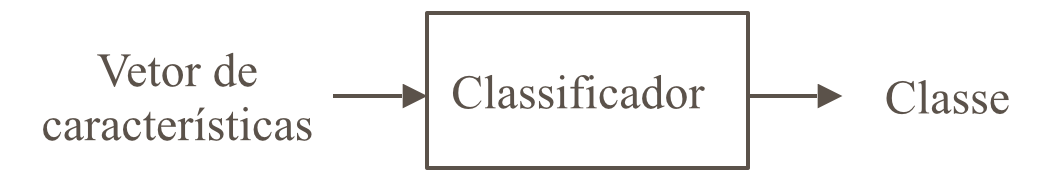
\includegraphics[width=0.7\textwidth]{imgs/classificador}
  \caption{Representação de classificador como uma função de bloco}
  \label{fig:classificador}
\end{figure}

Os tipos de classificadores utilizados neste trabalho serão discutidos com mais detalhes na seção \ref{sec:classificacao}.

Para composição do modelo de aprendizagem, uma base de dados de treinamento é utilizada. Esta base deve possuir uma quantidade significativa e com boa representatividade das classes envolvidas no problema. Normalmente se usa uma parte da base de dados de treinamento para validação do modelo de aprendizado (validação cruzada) ou mesmo uma base de dados diferente (base de testes ou validação), para que indicadores de qualidade do modelo possam ser avaliados. A seção \ref{sec:avaliacao} discorre sobre os métodos de avaliação utilizados neste trabalho.

Técnicas de aprendizagem de máquina podem ser utilizadas para encontrar padrões em diversos domínios, inclusive em imagens. É neste ponto que a disciplina de aprendizagem de máquina, advinda da área de inteligência artificial, se encontra com a disciplina de reconhecimento de padrões, advinda da área de processamento de sinais. Segundo \citeonline{jain:1989}, o fluxo padrão para soluções de reconhecimento de padrões consiste em três etapas:

\begin{enumerate}
    \item Filtragem e pré-processamento da entrada;
    \item Extração e seleção de características;
    \item Classificação.
\end{enumerate}


\subsection{Filtragem e Pré-processamento}

A etapa de filtragem e pré-processamento é responsável pela escolha e montagem da base de dados que será usada no processo de aprendizagem. A base deve conter uma quantidade significativa de exemplos de todas as classes envolvidas no problema.

Em aprendizado relacionado a imagens, essa etapa é comumente a responsável por normalizar e salientar as características desejadas nas amostras (realce de imagens, filtragem, etc). Exemplos irrelevantes, distorcidos ou repetidos também são eliminados durante a filtragem.

O objetivo principal desta etapa é preparar a base de dados para as etapas seguintes.


\subsection{Extração de Características}

A extração de características é feita selecionando os atributos oriundos dos dados (imagens, no trabalho em questão), a fim de encontrar as características úteis para o processo de reconhecimento. Essa etapa é crítica ao sucesso do aprendizado, uma vez que bons algoritmos de aprendizado só obtém êxito com uma bom conjunto de características relevantes ao problema.

Em projetos que envolvem classificação de imagens, uma gama de atributos podem ser extraídos, e podem ser descritos pelo nível da informação que representam. Nesta etapa há uma forte contribuição da disciplina de processamento digital de imagens \cite{gonzalez:2002}, que descreve filtragens, transformações e outras técnicas capazes de extrair informações sobre uma imagem ou pedaços dela.

Segundo \citeonline{nixon:2008}, informações de baixo-nível como bordas, histogramas de intensidade e coloração, são úteis para o reconhecimento de padrões em imagens, assim como características de níveis mais altos, como texturas, transformadas de Hough e extração de regiões conectadas.

O produto desta etapa é a representação de cada exemplo da base de dados em um vetor de características, de forma que possa ser usado por um ou mais classificadores em uma etapa futura.


\subsection{Classificação}\label{sec:classificacao}

Nesta etapa, todas as amostras de treinamento são classificadas e um modelo de aprendizado é gerado. Posteriormente ao processo de aprendizado, é nesta mesma etapa que as amostras não classificadas receberão uma classe dentre as envolvidas no problema. É neste momento que podemos comparar o desempenho de diferentes algoritmos de aprendizado para o conjunto de características escolhido para representar o problema.

Pode-se usar múltiplos classificadores mais simples, ao invés de apenas um mais robusto. Esta abordagem é chamada de sistemas com múltiplos classificadores (do inglês \textit{multiple classifier systems}) e podem ser compostos por classificadores do mesmo tipo (denominado \textit{Ensemble} de classificadores) ou de diferentes tipos.

São muitos os exemplos de classificadores que existem na literatura. Alguns dos mais utilizados são: classificadores estatísticos, redes neurais artificiais, árvores de decisão, máquinas de vetores de suporte, KNN, etc \cite{jain:1989}. 

%\subsubsection{Árvores de decisão}

%Árvores de decisão são considerados algoritmos de aprendizagem simbólica.


%Decision tree learning uses a decision tree as a predictive model which maps observations about an item to conclusions about the item's target value. It is one of the predictive modelling approaches used in statistics, data mining and machine learning. Tree models where the target variable can take a finite set of values are called classification trees. In these tree structures, leaves represent class labels and branches represent conjunctions of features that lead to those class labels. Decision trees where the target variable can take continuous values (typically real numbers) are called regression trees.

%In decision analysis, a decision tree can be used to visually and explicitly represent decisions and decision making. In data mining, a decision tree describes data but not decisions; rather the resulting classification tree can be an input for decision making. This page deals with decision trees in data mining.

%Decision tree learning is a method commonly used in data mining.[1] The goal is to create a model that predicts the value of a target variable based on several input variables. An example is shown on the right. Each interior node corresponds to one of the input variables; there are edges to children for each of the possible values of that input variable. Each leaf represents a value of the target variable given the values of the input variables represented by the path from the root to the leaf.

%A decision tree is a simple representation for classifying examples. Decision tree learning is one of the most successful techniques for supervised classification learning[citation needed]. For this section, assume that all of the features have finite discrete domains, and there is a single target feature called the classification. Each element of the domain of the classification is called a class. A decision tree or a classification tree is a tree in which each internal (non-leaf) node is labeled with an input feature. The arcs coming from a node labeled with a feature are labeled with each of the possible values of the feature. Each leaf of the tree is labeled with a class or a probability distribution over the classes.

%Os algoritmos utilizados em problemas de classificação podem ser categorizados em:

%\begin{itemize}
%	\item \textbf{Probabilísticos}:
%	\item \textbf{Geométicos}:
%	\item \textbf{Simbólicos}:
%\end{itemize}

%Existe uma grande variedade de algoritmos de aprendizagem de máquina propostos na literatura tais como Árvores de Decisão, k Vizinhos mais Próximos (kNN), Redes Neurais Artificiais, Support Vector Machines (SVM), etc. [Santos, 2008]. Além desses métodos individuais, os algoritmos de aprendizagem de máquina podem também ser combinados em conjuntos de classificadores [Dietterich, 2000].


\subsection{Avaliação}\label{sec:avaliacao}

Tanto durante o desenvolvimento de uma solução, quanto após sua execução em ambiente de produção, é preciso aferir ou quantificar o desempenho de um classificador. Isso é útil para determinar a qualidade do modelo criado, se o modelo continua adequado, bem como inspecionar se os atributos escolhidos são adequados para a classificação dos exemplos.

Comumente, o percentual de acerto obtido na classificação das amostras é um importante parâmetro para medir o desempenho do modelo. Este parâmetro é conhecido como acurácia ou taxa de reconhecimento. O oposto da acurácia é conhecido como taxa de erro.

De grande importância também é a composição da matriz de confusão (tabela \ref{tab:matrixConfusao}). Nela pode-se avaliar como um modelo está se comportando em termos de falsos positivos (um exemplo é classificado como pertencente à classe C, mas não é) e falsos negativos (um exemplo é atribuído a outra classe, mas deveria ser da classe C). A principal função desta matriz é a dar possibilidade de pensar sobre o custo dos erros, ou seja, mesmo que a taxa de acerto para o problema seja alto, uma ou mais classes do problema pode ter uma taxa de acerto bem abaixo do esperado.

\begin{table}[h]
  \centering
  \begin{tabular}{cccc}
  \multicolumn{2}{c}{\textbf{Resultado obtido}}                  &                               &                                              \\ \cline{1-2}
  \multicolumn{1}{|c|}{Classe A} & \multicolumn{1}{c|}{Classe B} &                               &                                              \\ \cline{1-3}
  \multicolumn{1}{|c|}{TP}       & \multicolumn{1}{c|}{FN}       & \multicolumn{1}{c|}{Classe A} & \multirow{2}{*}{\textbf{Resultado esperado}} \\ \cline{1-3}
  \multicolumn{1}{|c|}{FP}       & \multicolumn{1}{c|}{TN}       & \multicolumn{1}{c|}{Classe B} &                                              \\ \cline{1-3}
  \end{tabular}
  \caption{Um modelo de matriz de confusão}
  \label{tab:matrixConfusao}
\end{table}

Alguns valores podem ser obtidos através desta matriz. A própria acurácia do modelo pode ser obtida com a seguinte equação:

\begin{equation}
  Acurácia = \frac{TP+TN}{TP+FP+TN+FN}
\label{eq:acuracia}
\end{equation}

Ainda é possível obter a precisão e revocação. A precisão é o número de elementos relevantes recuperados dividido pelo número total de elementos recuperados (equação \ref{eq:precisao}) enquanto a revocação é definida como o número de elementos relevantes recuperados dividido pelo número total de elementos relevantes existentes, que deveriam ter sido recuperados (equação \ref{eq:revocacao}).

\begin{equation}
  Precisão = \frac{TP}{TP+FP}
\label{eq:precisao}
\end{equation}


\begin{equation}
  Revocação = \frac{TP}{TP+FN}
\label{eq:revocacao}
\end{equation}

\section{Segmentação de imagens}

O processo de segmentação subdivide uma imagem em suas várias regiões ou objetos. O nível em que a subdivisão é feita depende do problema a ser resolvido, ou seja, a segmentação deve parar quando os objetos de interesse de uma aplicação forem isolados. Por exemplo, na inspeção automática de uma linha de montagem de produtos eletrônicos, o interesse reside em analisar imagens dos produtos com o objetivo de determinar a presença ou ausência de anomalias específicas, como componentes faltando ou conexões quebradas. Não há sentido em continuar segmentando além do nível de detalhes necessário para a identificação destes elementos.

Segmentação de imagens não-triviais é um dos problemas mais difíceis em processamento digital de imagens \cite{gonzalez:2002}. Algoritmos de segmentação geralmente se baseiam em uma das duas propriedades básicas de valores de intensidade dos pixels: descontinuidade e similaridade. Na primeira propriedade, a abordagem é particionar a imagem baseando-se em mudanças abruptas na intensidade dos pixels, como as bordas. A segunda categoria se baseia no particionamento de uma imagem em regiões que são similares de acordo com um critério em particular, que pode ser coloração, textura, entre outros.

Neste trabalho, conforme será descrito no capítulo \ref{cap:metodologia}, testamos uma série de atributos para determinar a melhor forma de segmentar as regiões das imagens aéreas da floresta amazônica, como uma das etapas da pesquisa de detecção de anomalias.
